\chapter{Jet Energy Scale}
\label{JES}

In order to easily compare experimental results with theoretical results they must be brought to the same scale.  
This is usually done by applying a calibration to experimental results to bring the measured signal back to `truth' scale, making the results detector independent.  
For jets the relation between this measured energy and the `truth' scale energy is known as the \gls{JES}.

\begin{figure}[!ht]
  \begin{center}
    \scalebox{0.40}{
      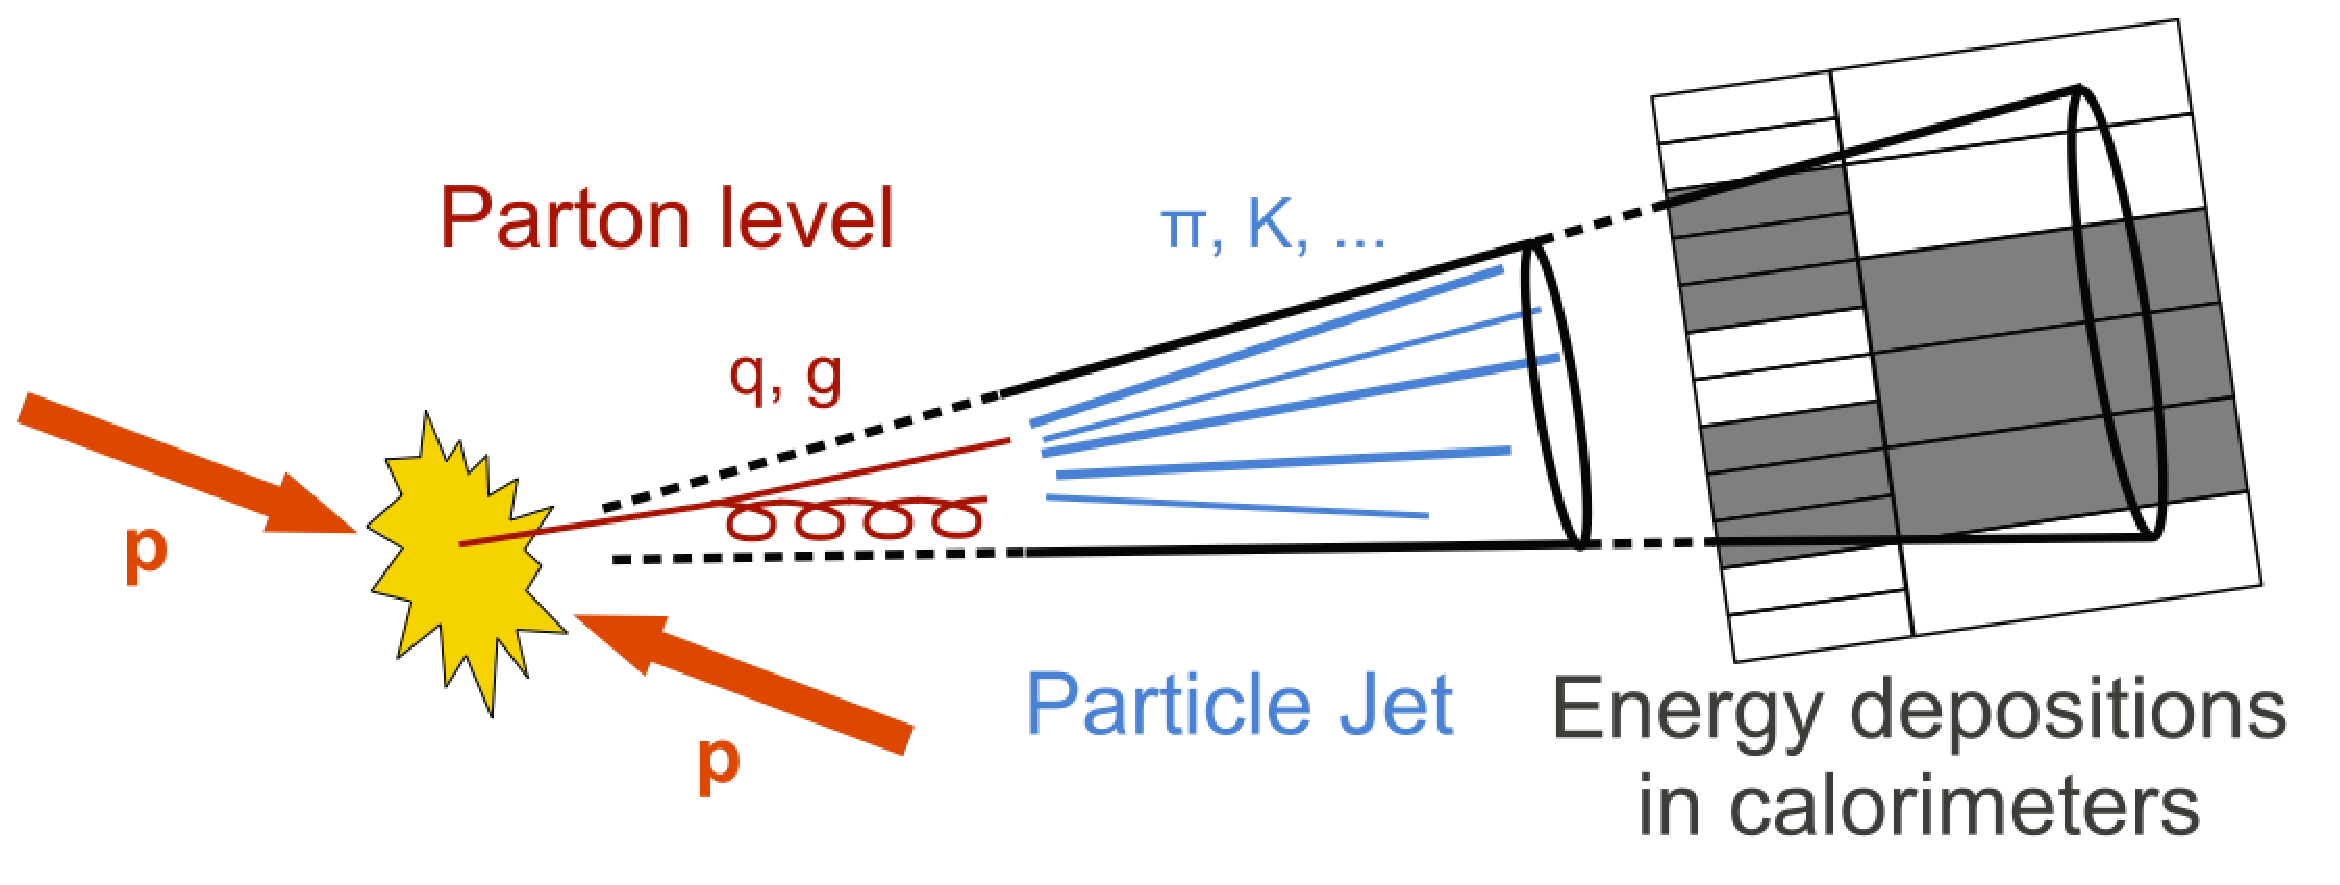
\includegraphics{plots/Chap3/Sketch_PartonParticleCaloJet.eps}
    }
  \end{center}
  \caption[Jet showering evolution.]
      {\small A cartoon outlining the progression from parton level to a calorimeter jet.}
  \label{JetLevelsFig}
\end{figure}


\section{Jet Energy Scale in ATLAS}
\label{ATLASJES}

\section{Jet Response}

\section{$E_T^{miss}$ Projection Method}
\label{METProj}

%\subsection{Biases}

%Combinations of physics and detector effects may affect the measurement of the MPF.  
%For example both final state radiation (FSR) and initial state radiation (ISR) will affect the assumption of momentum balance in Eq.~\ref{Assume1}.  
%Both ISF and FSR have the effect of making the Z and the jet not back-to-back in the transverse plane, i.e. $\Delta\phi < \pi$.  
%This allows events where radiation will have a large effect on the response to be cut out by requiring that $\Delta\phi > 2.9$.  
%These events may be further suppressed by rejecting events with any highly energetic secondary jets.  







